\documentclass{article}

\usepackage{graphics}
\usepackage{graphicx}
\usepackage[a4paper,
            top=2cm,
            bottom=3cm,
            left=3cm,
            right=2cm,
            marginparwidth=1.75cm
            ]{geometry}

\usepackage{float}

\title{TP01 - Estrutura de dados}
\author{Marcos Daniel Souza Netto - 2022069492} 
\date{\today}

\begin{document}
\maketitle

\section{Introdução}

O problema proposto foi dividido em duas partes: primeira, a implementação 
de um solucionador de equações booleanas dado o valor das variáveis; segunda,
a implementação de um solucionador SAT (Verificar se a esquação é satisfazível) 
com a restrição de no máximo cinco quantificadores.

\section{Método}

A seguir serão detalhados a implementação da soluções, de modo a explicitar 
as estruturas de dados utilizadas e as estratégias de solução. A priori vale 
apresentar as especificações do ambiente de desenvolvimento utilizado:

\begin{itemize}
    \item Sistema Operacional: Ubuntu 22.04.3 LTS;
    \item Compilador: G++ 11.4.0;
    \item Processador: Ryzen 5 5500u;
    \item Memória RAM: 8GB.
\end{itemize}


\subsection{Estruturas de dados}

Em síntese, foram utilizadas as seguintes estruturas de dados:

\begin{itemize}
    \item \textbf{Stack}: Representa uma pilha de elementos, sendo utilizada em diversos trechos do código, como por exemplo para percorrer a árvore de soluções e para transformar a expressão infixa (Na ordem habitual que estamos acostumados, como por exemplo $a \lor b$) para a forma posfixa ($a b \lor$);
    \item \textbf{Binary Tree}: Representa uma árvore binária, sendo utilizada para representar a árvore de soluções na parte 2 do trabalho;
\end{itemize}

A implementação dessas estruturas se localizam nos arquivos \textit{stack.h} e \textit{binary\_tree.h}.

\subsection{Classes e principais funções}
O código foi dividido em três grandes classes, sendo elas:
\begin{itemize}
    \item \textbf{stack.h}: Implementação da estrutura de dados pilha, e contém as principais operações de uma pilha, como \textit{push}, \textit{pop}, \textit{top}, \textit{isEmpty} e \textit{size}, que respectivamente realiza a inserção de um elemento, a remoção do elemento do topo, retorna o elemento do topo, verifica se a pilha está vazia e retorna o tamanho da pilha; 
    \item \textbf{binary\_tree.h}: Implementação da estrutura de dados árvore binária, e contém a definição de nó dessa árvore além das principais operações em árvore, como a inserção de filhos à esquerda ou à direita de um nó, e o caminhamento na árvore, que pode ser feito em pré-ordem, em ordem ou em pós-ordem;
    \item \textbf{utils.h e utils.cpp}: São respectivamente, definição e implementação das principais funções de manipulação das estruturas de dados utilizadas para a solução do problema.
        \subitem \textbf{infixToPostfix(string infix)}: Recebe uma string contendo uma expressão booleana na forma infixa e retorna uma string contendo a mesma expressão na forma posfixa;
        \subitem \textbf{evaluatePostfix(string postfix, int arr[])}: Recebe uma string contendo uma expressão booleana na forma posfixa e um vetor contendo os valores das variáveis da expressão(0 $\to$ false e 1 $\to$ true) e retorna o resultado da expressão(0 $\to$ false ou 1 $\to$ true);
        \subitem \textbf{satTree(string postfix, string vals)}: Recebe uma string contendo uma expressão booleana na forma posfixa, um vetor contendo os valores das variáveis da expressão(0 $\to$ false, 1 $\to$ true, e $\to$ existe, a $\to$ para todo) e retorna 1 ou 0 caso a expressão seja satisfazível ou não, respectivamente. Caso ela seja satisfazível, uma string contendo a possível solução é retornada;
    \item \textbf{main.cpp}: Contém a função principal do programa, que realiza a leitura dos dados de entrada e chama as funções de solução do problema.   
\end{itemize}

\section{Análise de Complexidade}

A seguir serão apresentadas as análises de complexidade das principais funções do programa.

\subsection{infixToPosfix}
Como mencionado acima, esta função converte uma expressão infixa para a representação posfixa. Para isso, a função percorre a string contendo a expressão infixa, e para cada caractere, verifica se ele é um operando ou um operador. Caso seja um operando, ele é adicionado à string de saída, caso seja um operador, ele é adicionado à pilha. Ao final da leitura da string, todos os operadores que estão na pilha são adicionados à string de saída. Portanto, a complexidade da função é $O(n)$, onde $n$ é o tamanho da string de entrada.

A complexidade de espaço é $O(n)$, pois a pilha pode conter no máximo $n$ elementos.

\subsection{evaluatePostfix}
Esta função recebe uma string contendo uma expressão booleana na forma posfixa e um vetor contendo os valores das variáveis da expressão e retorna o resultado da expressão. Para isso, a função percorre a string de entrada, e para cada caractere, verifica se ele é um operando ou um operador. Caso seja um operando, ele é adicionado à pilha, caso seja um operador, ele é removido dois operandos do topo da pilha ou apenas um operando (No caso do operador $\sim$), e o resultado da operação é adicionado à pilha. Ao final da leitura da string, o resultado da expressão é o elemento que está no topo da pilha. Portanto, a complexidade da função é $O(n)$, onde $n$ é o tamanho da string de entrada.

A complexidade de espaço é $O(n)$, pois assim como a função anterior, a pilha pode conter no máximo $n$ elementos.

\subsection{satTree}
Esta função recebe uma string contendo uma expressão booleana na forma posfixa, um vetor contendo os valores das variáveis da expressão(agora podendo conter quantificadores existe e para todo) e retorna 1 ou 0 caso a expressão seja satisfazível ou não, respectivamente. Caso ela seja satisfazível, uma string contendo a possível solução é retornada. 

Para isso, a função indexa os quantificadores da expressão, em seguida percorre o vetor dos quantificadores construindo a árvore de solução pelos últimos quantificadores até o primeiro.
A árvore possui, portanto, como folhas os possíveis valores para os quantificadores (0 ou 1) e desse modo ela possui $2^k$ folhas, onde $k$ é o número de quantificadores, seja existe ou para todo. Para exemplificar considere a figura \ref{fig:sat_tree}.

\begin{figure}[H]
    \centering
    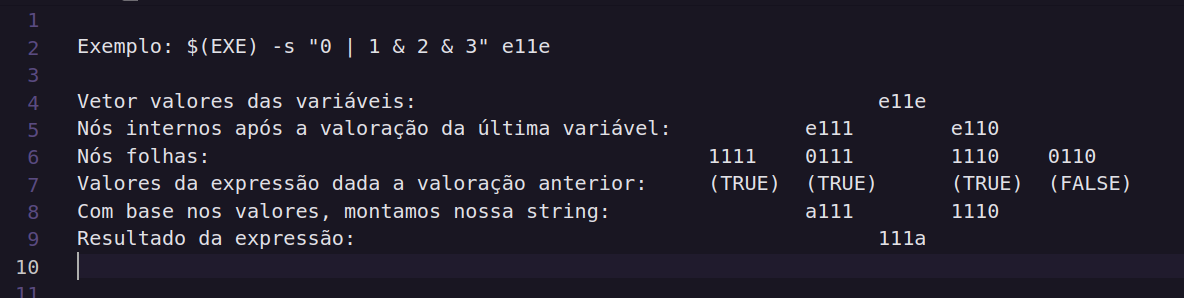
\includegraphics[width=\textwidth]{./images/sat_tree.png}
    \caption{Árvore de solução para a expressão $\exists a \exists d , b = c = 1,  (a \lor b \land c \land d)$}
    \label{fig:sat_tree}
\end{figure}

Como visto, a árvore possui $2^k$ folhas, e para cada uma delas, a função \textit{evaluatePostfix} é chamada para verificar se a expressão é satisfazível. Portanto, a complexidade da função é $O(2^k)$, onde $k$ é o número de quantificadores.

Já a complexidade de espaço é $O(k)$, pois a solução da árvore é realizada de modo ir o mais profundo na árvore possível, e cada vez que um nó é resolvido, seus filhos são removidos da memória.
\section{Estratégias de robustez}

\section{Análise Experimental}

A seguir serão apresentados os resultados obtidos na experimentação do programa.

\subsection{Localidade de Referência}

Utilizando o programa analisamem, fornecido pelo professor, foi possível observar a localidade de referência do programa. Importante notar que aqui serão apresentadas imagens relacionadas a parte de satisfatibilidade do programa, afinal utiliza a parte de solucionador de equaações booleanas como subrotina.

\begin{figure}[H]
    \centering
    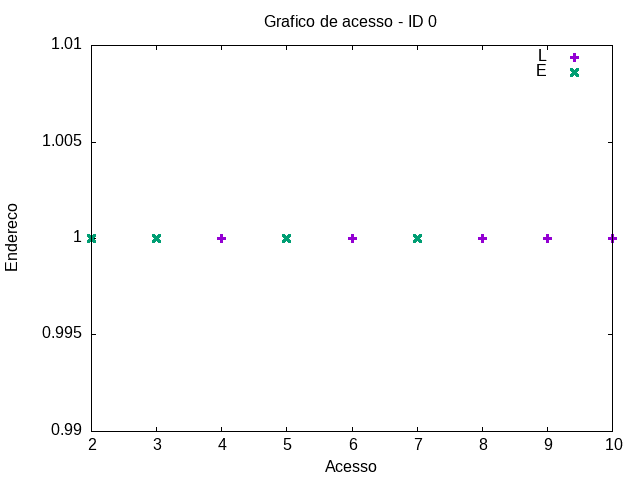
\includegraphics[width=0.5\textwidth]{./images/sat_tree/registro_s-acesso-0.png}
    \caption{any}
    \label{fig:loc_ref_1}
\end{figure}

\subsection{Tempo de execução}

Nesse experimento foi realizado medições de tempo de execução a parte de satisfatibilidade do programa, variando o número de quantificadores da expressão. Para isso,
variamos a quantidade de quantificadores da expressão de 13 até 20, para que possamos observar o comportamento do programa para um número maior de quantificadores.
Teve como base o seguinte comando (Atente-se que estamos variando o número de quantificadores): 


\verb#bin/tp01 -s "0 | 1 | 2 | (...) | 17 | 18 | 19" eeeeeeeeeeeeeeeeeeee#

\begin{figure}[H]
    \centering
    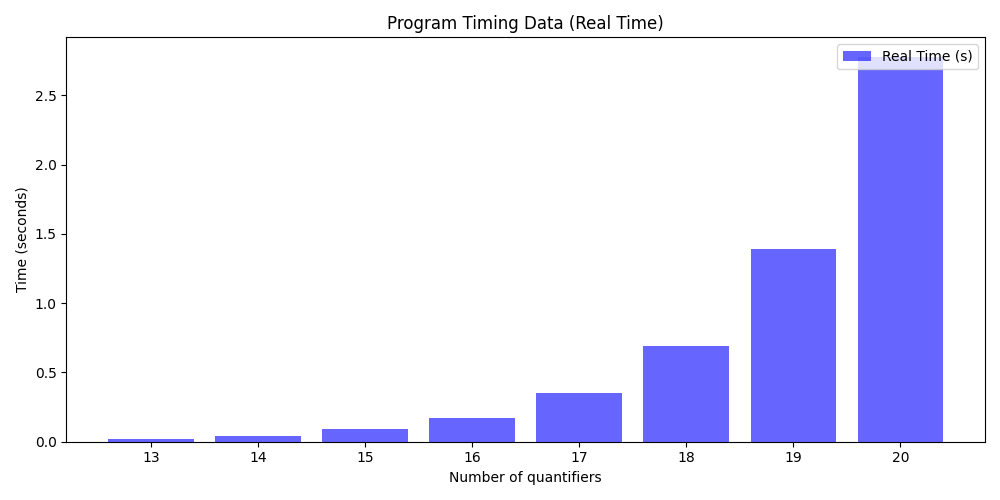
\includegraphics[width=\textwidth]{./images/time.png}
    \caption{Tempo de execução do programa para diferentes números de quantificadores}
    \label{fig:time}
\end{figure}

\section{Conclusões}

\section*{Bibliografia}

Slides da disciplina de Estrutura de Dados, ministrada pelo Prof. Wagner Meira Jr. e Prof. Eder Fereira Figuiredo.


\section*{Instruções para compilação e execução}

Em um terminal, navegue até a pasta raiz do projeto e execute os seguintes comandos:

\begin{verbatim}
    $ make
    $ ./bin/tp01 -a "<expressão booleana>" <valores das variáveis> // Valor 
    $ ./bin/tp01 -s "<expressão booleana>" <valores das variáveis> // SAT
\end{verbatim}

\end{document}